\chapter{Problema}
\label{chap:pre1}

Neste capítulo apresenta-se o problema que o presente trabalho visa resolver. O enunciado do problema, como o próprio nome indica, aborda o problema, descrevendo-o de forma concisa (Secção~\ref{sec:pre1_problem}). Essa descrição permite definir os objetivos do trabalho (Secção~\ref{sec:pre1_objectives}), complementando-os com âmbito e pressupostos associados (Secção~\ref{sec:pre1_objectives}). Por fim, estabelece-se a avaliação da solução, ou seja, as metodologias contempladas para avaliar o resultado obtido, bem como os critérios de sucesso a considerar para a avaliação final do trabalho (Secção~\ref{sec:pre1_solutionevaluation}).

\section{Enunciado do problema}
\label{sec:pre1_problem}

O conceito de \gls{mes}, um sistema que, além de gerir as operações dum determinado processo fabril, mantém dados relativos às diversas etapas inerentes ao processo em questão, está intrinsecamente relacionado com a Indústria 4.0, uma iniciativa que se destina a criar fábricas inteligentes, usando tecnologias como os \glspl{cps}, a \gls{iot} e \textit{Cloud Computing}~\parencite{intelligent_manufacturing_context_industry40_review}. O {\productname} é um destes sistemas. Contudo, a capacidade de adaptação às características dos utilizador é um requisito complexo, que nem sempre é passível de ser cumprido. Isso pode tornar o produto difícil de usar, numa perspetiva de acesso a informação relevante para o processo e de apoio à decisão. Por outras palavras, se o utilizador pretende efetuar uma determinada pesquisa, necessita de conhecer os detalhes da ferramenta a usar, ao invés de simplesmente \inquotes{pedir} (através de texto ou voz) ao sistema que lhe devolva o resultado.

\textbf{A conceção de um módulo de linguagem natural para interface com o {\productname}, permitindo a consulta e pesquisa de estados do processo de fabrico}, torna-se importante para o sistema, uma vez que possibilita o utilizador interagir com o sistema de uma forma simples, intuitiva, eficiente e natural, através de escrita.

\section{Objetivos}
\label{sec:pre1_objectives}
De uma maneira geral, com este trabalho pretende-se desenvolver uma solução baseada em linguagem natural que promova a interação do utilizador com o sistema \gls{mes}. Com o intuito de solucionar o problema enunciado na Secção~\ref{sec:pre1_problem}, definem-se os seguintes objetivos:

\begin{enumerate}
    \item
    \label{enum:pre1_objectives_1}
    {
        \textit{Contextualizar o problema numa perspetiva de negócio} -- análise detalhada do problema, as implicações que tem para negócio e para o produto \gls{mes}, descrevendo o valor intrínseco à solução (Capítulo~\ref{chap:Chapter2});
    }
    \item
    \label{enum:pre1_objectives_2}
    {
        \textit{Estudar soluções disponíveis no mercado e/ou bibliotecas de processamento de linguagem natural} -- obtenção de informação da área de conhecimento envolvida, de ferramentas semelhantes e de bibliotecas tipicamente usadas na implementação de tais módulos (Capítulo~\ref{chap:Chapter3});
    }
    \item
    \label{enum:pre1_objectives_3}
    {
        \textit{Definir a solução mais adequada, considerando as diversas opções apresentadas} -- comparação e avaliação das diversas opções identificadas (Capítulo~\ref{chap:Chapter3});
    }
    \item
    \label{enum:pre1_objectives_4}
    {
        \textit{Especificação da arquitetura do módulo} -- que permita responder aos requisitos definidos e antecipar soluções para possíveis problemas;
    }
    \item
    \label{enum:pre1_objectives_5}
    {
        \textit{Descrever a semântica de domínio} -- identificação dos domínios a explorar e construção de uma base de conhecimento semântico (\idest{um dicionário}) para o módulo;
    }
    \item
    \label{enum:pre1_objectives_6}
    {
        \textit{Desenvolvimento de prova de conceito} -- implementação da solução de acordo com a arquitetura conceptualizada;
    }
    \item
    \label{enum:pre1_objectives_7}
    {
        \textit{Prover a solução de um mecanismo de feedback para auto-aprendizagem} -- o que permitirá ao módulo adaptar-se às necessidades do utilizador, melhorando a qualidade das suas respostas. Numa fase inicial, este mecanismo consiste simplesmente em questionar o utilizador sobre a exatidão da resposta apresentada;
    }
    
    \item
    \label{enum:pre1_objectives_8}
    {
        \textit{Avaliar a qualidade da solução desenvolvida} -- com base nas estratégias de avaliação definidas em~\ref{enum:pre1_qualitystrategies}, concluir acerca da qualidade da solução e do contributo do trabalho para a resolução do problema;
    }
    \item
    \label{enum:pre1_objectives_9}
    {
        \textit{Elaboração da tese escrita} -- como forma de transmitir o conhecimento alcançado durante a elaboração do trabalho.
    }
\end{enumerate}

\section{Âmbito}

Embora os objetivos estejam definidos, surge a necessidade de explicitar sucintamente o âmbito do trabalho, bem como os pressupostos a ter em consideração. Por conseguinte, os seguintes assuntos não serão abordados:

\begin{itemize}
    \item
    {
        O enquadramento do problema com outros \glspl{mes}. Apenas é contemplada a realidade do problema no contexto do {\productname} (objetivo~\ref{enum:pre1_objectives_1});
    }
    \item
    {
        As soluções e bibliotecas de linguagem natural que não mostrem evidências de relevância para o problema, tendo em conta os critérios de preço, adesão da comunidade de desenvolvimento e respetiva complexidade (objetivo~\ref{enum:pre1_objectives_2});
    }
    \item 
    {
        A inclusão de diferentes domínios na solução desenvolvida (objetivos~\ref{enum:pre1_objectives_3}, \ref{enum:pre1_objectives_4} e \ref{enum:pre1_objectives_5});
    }
\end{itemize}

O termo \inquotes{Domínio} é empregue ao longo do texto para denotar um conjunto de características que descrevem uma família de conceitos comuns a um determinado processo. Por exemplo, duas empresas que produzem equipamentos médicos, apesar de poderem ter processos de fabrico diferentes, abordam o mesmo domínio.

Neste trabalho assume-se que a solução a desenvolver, embora pensada para integrar em diferentes processos de manufatura, é uma prova de conceito, pelo que deverá considerar um processo fabril (a ser definido) e consequentemente, lidar com a semântica específica desse domínio.

\section{Avaliação da Solução}
\label{sec:pre1_solutionevaluation}

A avaliação do resultado final é imprescindível para concluir acerca do sucesso do trabalho, permitindo perceber se a conjetura fundada a respeito da solução é aceite. Desse modo, especificam-se a metodologia de avaliação para solução desenvolvida e os critérios de sucesso a serem considerados.

\subsection{Metodologia de Avaliação}
Com o propósito de perceber se a solução desenvolvida é adequada para o {\productname} e para o utilizador final, definem-se as seguintes estratégias para a metodologia de avaliação deste trabalho:

\begin{enumerate}
\label{enum:pre1_qualitystrategies}
    \item 
    {
        \textit{Garantir que a solução analisa e responde corretamente a um conjunto de perguntas pré-definidas} -- a solução deverá responder adequadamente a um conjunto limitado de perguntas:
        \begin{itemize}
            \item 
            {
                Quantas operações foram executadas por semana, durante o mês $M$?
            }
            \item
            {
                Qual o número de operações $O$ por produto e turno, durante o mês $M$?
            }
            \item
            {
                Qual a média de $X$ de operações $O$, no passo $P$ do processo, por turno, no mês $M$? 
            }
            \item
            {
                Qual o número de materiais cujo valor de $X$ é inferior a $Y$, para o passo $P$ do processo, agrupando por $G$?
            }
        \end{itemize}
        
        Nas questões apresentadas, as letras representam as variáveis próprias do domínio, que o utilizador conhece e que o sistema deve ser capaz de reconhecer.
    }
    \item
    {
        \textit{Usar as respostas recolhidas pelo mecanismo de feedback para conclusão acerca da usabilidade da solução} -- as respostas fornecidas pelo utilizador permitirão perceber se a solução contempla as suas necessidades e quais as medidas ou requisitos podem ser futuramente implementados, com a perspetiva de melhorar a qualidade do sistema.
    }
\end{enumerate}

Ambas estratégias possibilitam perceber a adequabilidade da solução para o produto e para o utilizador, quer numa perspetiva de facilidade de utilização, quer na exatidão da resposta dada.

\subsection{Critérios de Sucesso}

De seguida, enumeram-se os critérios de sucesso para o trabalho, associados aos respetivos objetivos:

\begin{enumerate}
    \item
    {
        \textit{A solução apresentada é extensível a outros domínios e facilmente integrada no {\productname}} -- garante-se assim que a arquitetura especificada considerou diversos domínios, facilidade e capacidade de integração com o produto, ainda mesmo sendo um protótipo (objetivos~\ref{enum:pre1_objectives_3}, \ref{enum:pre1_objectives_4} e \ref{enum:pre1_objectives_6});
    }
    \item
    {
        \textit{Prova de conceito dá resposta correta ao domínio definido} -- que implica responder corretamente às questões listadas em \ref{enum:pre1_qualitystrategies}, garantindo que semântica foi bem definida e que o requisito de qualidade está cumprido (objetivos~\ref{enum:pre1_objectives_5}, \ref{enum:pre1_objectives_6}, \ref{enum:pre1_objectives_7} e \ref{enum:pre1_objectives_8}).
    }
    \item 
    {
        \textit{Tese escrita} -- na qual se abordam o problema, o contexto no qual se insere e o valor que traz ao produto final. Deve conter o estado da arte, apresentando a revisão da literatura existente, focando nas soluções semelhantes e/ou ferramentas relevantes que perspetivam estratégias de solução para o problema. Por fim, descreve-se a solução proposta, contemplando cada uma das fases inerentes ao seu desenvolvimento (visão, análise, desenho e implementação) e faz-se a conclusão acerca do trabalho (todos os objetivos descritos em~\ref{sec:pre1_objectives});
    }
\end{enumerate}

% ----------------------------------------
% CONTRIBUIÇÕES
% ----------------------------------------
\subsection{Contribuições Esperadas}

O trabalho a ser desenvolvido pretende providenciar uma solução para o problema descrito anteriormente (Secção \ref{sec:pre1_problem}). Não se aspira fornecer uma solução definitiva, espera-se sim, contribuir com conhecimento de carácter teórico e prático (\idest{um protótipo}), que possibilite a integração futura de uma nova funcionalidade num produto já existente, trazendo-lhe mais-valia funcional, destacando-o dos seus concorrentes. No decorrer deste trabalho serão abordados temas relativos a \gls{mes}, a \gls{ia}, especificamente \gls{pln}, e \textit{Business Intelligence}.

Resumidamente, as contribuições esperadas são a seguir enunciadas:

\begin{itemize}
    \item
    {
        Estado da arte no domínio de Processamento de Linguagem Natural, aplicadas à conversão de texto para \gls{sql} e sistemas análogos à solução a desenvolver;
    }
    \item 
    {
        Documentação dos requisitos de sistema, incluindo análise e desenho, constando os respetivos artefactos de \gls{uml};
    }
    \item 
    {
        Dicionário semântico do domínio a ser definido para o módulo;
    }
    \item
    {
        Especificação e desenvolvimento do protótipo, considerando a futura integração com o sistema {\productname};
    }
    \item
    {
        Conceção do mecanismo de \textit{feedback} permitindo a adaptação ao utilizador e consequentemente, a auto-aprendizagem do sistema.
    }
\end{itemize}

De uma forma geral, é realçada a contribuição para o avanço do conhecimento no domínio da \gls{ia}, mais especificamente na área da \gls{pln}, aplicada ao contexto dos sistemas \gls{mes} e que servirá como base para a integração duma solução deste tipo no {\productname}.

% ----------------------------------------
% METODO DE TRABALHO
% ----------------------------------------
%\chapter{Método de trabalho}
%\label{chap:pre3}
%\textit{A definir}

% ----------------------------------------
% CONTEXTO
% ---------------------------------------- 
\chapter{Contexto}
\label{chap:Chapter2}

\textit{A definir}

\section{A Empresa}
\label{sec:chap2_company}

A {\companyname} é uma empresa fundada em 2009, com sede e centro de engenharia na Maia (Porto, Portugal), subsidiárias em Dresden (Alemanha), Suzhou (China), Austin (Estados Unidos da América) e um escritório comercial em Taiwan. O objetivo é proporcionar à indústria uma solução de gestão e controlo de produção, procurando reduzir os custos de produção, flexibilizar para satisfazer a procura e capacitar a organização de uma maior agilidade, visibilidade e fiabilidade~\parencite{cmf_overview}. O compromisso da empresa~\parencite{cmf_overview} foca-se no desenvolvimento de~\inquotes{soluções de vanguarda, indo de encontro aos desafios mais importantes da indústria e disponibilizar à lista crescente de clientes satisfeitos, soluções de elevado valor acrescentado, no prazo e orçamento requerido}\footnote{Tradução livre do autor. No original~\inquotes{[...] solutions that address the most urgent industry challenges and provide our growing list of satisfied customers with the highest value solution, on-time and on-budget.}.}.

A estratégia da empresa está sintetizada na sua missão, visão e valores. Se a missão descreve a razão da empresa existir, ou seja, o seu propósito, já a visão retrata o que se aspira alcançar. Isto posto, a missão e visão são divulgados a seguir~\parencite{cmf_strategy}: 

\begin{itemize}
    \item 
    {
        \textit{Missão} -- \inquotes{trazer valor através da convergência de inteligência, operações e tecnologias de automação para a Indústria 4.0.}\footnote{Tradução livre do autor. No original \inquotes{We drive business value through the convergence of intelligence, operations, and automation technologies for Industry 4.0.}.}.
    }
    \item 
    {
        \textit{Visão} -- \inquotes{Tornar a Indústria 4.0 uma realidade para todos fabricantes.}\footnote{Tradução livre do autor. No original \inquotes{We will make Industry 4.0 a reality for all manufacturers.}.}.
    }
\end{itemize}

Relativamente aos valores, são estes que suportam a visão, moldam a cultura empresarial e são a essência da sua identidade. Como tal, de seguida apresentam-se os valores da Critical Manufacturing~\parencite{cmf_strategy}:

\begin{itemize}
    \item 
    {
        \textit{Inovação} -- \inquotes{Exceder as expectativas dos clientes através das soluções mais eficientes e de mais alto valor para indústria.}\footnote{Tradução livre do autor. No original \inquotes{We constantly exceed our customers’ expectations through the most efficient and high value-added manufacturing solutions.}.}.
    }
    \item
    {
        \textit{Agilidade} -- \inquotes{Adaptar as pessoas, processos e soluções de forma a responder à evolução do mundo da manufatura de alta tecnologia.}\footnote{Tradução livre do autor. No original \inquotes{We continuously adapt our people, processes and solutions to respond to the evolving world of high-tech manufacturing.}.}.
    }
    \item
    {
        \textit{Compromisso} -- \inquotes{Defender o sucesso contínuo dos clientes e da empresa.}\footnote{Tradução livre do autor. No original \inquotes{We champion the continued success of our customers and our company.}.}.
    }
\end{itemize}

Por conseguinte, com base na sua estratégia, o presente trabalho pretende demonstrar viabilidade e o valor da utilização da \gls{IA}, nomeadamente na área do \gls{PLN}, para a interação com o Critical Manufacturing MES e obter informação pertinente para o utilizador final. 

\section{O Produto}
\label{sec:chap2_product}

\textit{A definir}

\section{Análise de Valor}
\label{sec:chap2_valueanalysis}

\textit{A definir}

% ----------------------------------------
% ESTADO DA ARTE
% ---------------------------------------- 
% Chapter 3

\chapter{Estado da Arte}
\label{chap:Chapter3}

%----------------------------------------------------------------------------------------
%	
%----------------------------------------------------------------------------------------


% ----------------------------------------
% PROPOSTA DE SOLUÇÃO
% ---------------------------------------- 
% Se necessário....

% ----------------------------------------
% PLANO DE TRABALHO
% ---------------------------------------- 
\chapter{Plano e Método de Trabalho}
\label{chap:pre7}

Um plano de trabalho é uma ferramenta importante na gestão de qualquer projeto, na medida em que permite ter visibilidade da sua extensão temporal, das tarefas a realizar e do período associado a cada uma delas. Na Figura~\ref{fig:planning-gantt_chart} demonstra-se o diagrama de \textit{Gantt}, contendo as tarefas inerentes a cada uma das fases do projeto, descriminadas na tabela abaixo.

\begin{table}[!ht]
\caption{Fases do projeto, periodicidade e respetiva duração}
\label{tab:project-phases}
\centering
\resizebox{\textwidth}{!}{\begin{tabular}{l|l|l|l}
%
\toprule
%
\tabhead{Fase do Projeto}&\tabhead{Data Prevista de Início}&\tabhead{Data Prevista de Fim}&\tabhead{Duração (dias)}\\ 
%
\midrule
Conceção                 & 01-Jan-2019                      & 16-Fev-2019                   & 46                      \\
Análise                  & 11-Fev-2019                      & 08-Março 2019                 & 25                      \\
Desenvolvimento          & 04-Março-2019                    & 17-Maio-2019                  & 74                      \\
Validação                & 17-Maio-2019                     & 12-Junho-2019                 & 26                      \\
Documentação             & 01-Jan-2019                      & 30-Junho-2019                 & 180                     \\ 
%
\bottomrule
\end{tabular}}
\end{table}

A Tabela~\ref{tab:project-phases} carece de informação sucinta de cada uma das fases, pelo que se passam a descrever:

\begin{itemize}
    \item 
    {
        \textit{Conceção} -- engloba as tarefas que relacionadas com o problema, o seu enquadramento, o estudo do valor e estado da arte. Ou seja, a visão do projeto;
    }
    \item
    {
        \textit{Análise} -- nesta fase, faz-se o levantamento dos requisitos, a escolha e definição da semântica de domínio, estipulam-se a(s) tecnologia(s) a utilizar e especifica-se a arquitetura para o módulo. A presente fase consiste no estudo e preparação para o desenho da solução; 
    }
    \item
    {
        \textit{Desenvolvimento} -- desenvolve-se a solução conjeturada na fase anterior, envolvendo um período de experimentação de código base da arquitetura definida (para possível reestruturação ou ajuste);
    }
    \item
    {
        \textit{Validação} -- avalia-se a solução com base nos critérios definidos na secção~\ref{sec:pre1_solutionevaluation} e consequentemente, podem-se registar melhorias para o módulo. É nesta fase que também se demonstra a solução às partes interessadas do trabalho (\exempligratia{\gls{ceo}, \gls{cto}, {\supname}, orientador do projeto, {\cosupname}, responsável pelo projeto etc.});
    }
    \item
    {
        \textit{Documentação} -- engloba a escrita da tese como veículo de transmissão de conhecimento obtido e de outros documentos de suporte, a serem usados no contexto empresarial (\exempligratia{documento de especificação de requisitos de \textit{software}, especificação arquitetural de \textit{software}, manual de instalação e outros que façam sentido}).
    }
\end{itemize}

Quanto ao método de trabalho a seguir na realização deste trabalho, são considerados os seguintes passos:

\begin{enumerate}
    \item 
    {
        \textit{Revisão de literatura disponível sobre o contexto do problema} -- com o objetivo de perceber o estado atual do {\productname} e as implicações que o módulo trará, assim como concluir acerca do valor da solução para o produto;
    }
    \item
    {
        \textit{Revisão de literatura existente acerca de \gls{pln} e paradigmas arquiteturais relacionados} -- adquirir conhecimentos sobre técnicas e ferramentas de \gls{pln}, principalmente analisando soluções já existentes, identificando aspetos relevantes para o trabalho e outros que não foram contemplados;
    }
    \item
    {
        \textit{Idealização do módulo} -- depois da análise dos conhecimentos adquiridos com as revisões realizadas nos passos descritos anteriormente, parte-se para o levantamento dos requisitos junto das partes interessadas do projeto, resultando na concepção de um módulo capaz de lhes dar resposta; 
    }
    \item
    {
        \textit{Estudo do domínio de negócio} -- com o intuito de entender a semântica do negócio em questão e definir um dicionário a ser usado pela solução;
    }
    \item
    {
        \textit{Implementação do módulo e validação} -- o foco é pôr em prática a solução conceptualizada nas fases anteriores. Após a implementação, são realizam-se testes com vista a perceber se os resultados obtidos são os esperados e proceder às melhorias que forem evidentes;
    }
    \item
    {
        \textit{Elaboração da documentação} --  por fim, passa-se à escrita do presente documento e de documentos de suporte, baseando-se nas observações, nas experiências e conclusões obtidas ao longo do projeto.
    }
\end{enumerate}

\clearpage
\begin{sidewaysfigure}[!ht]
    \centering
    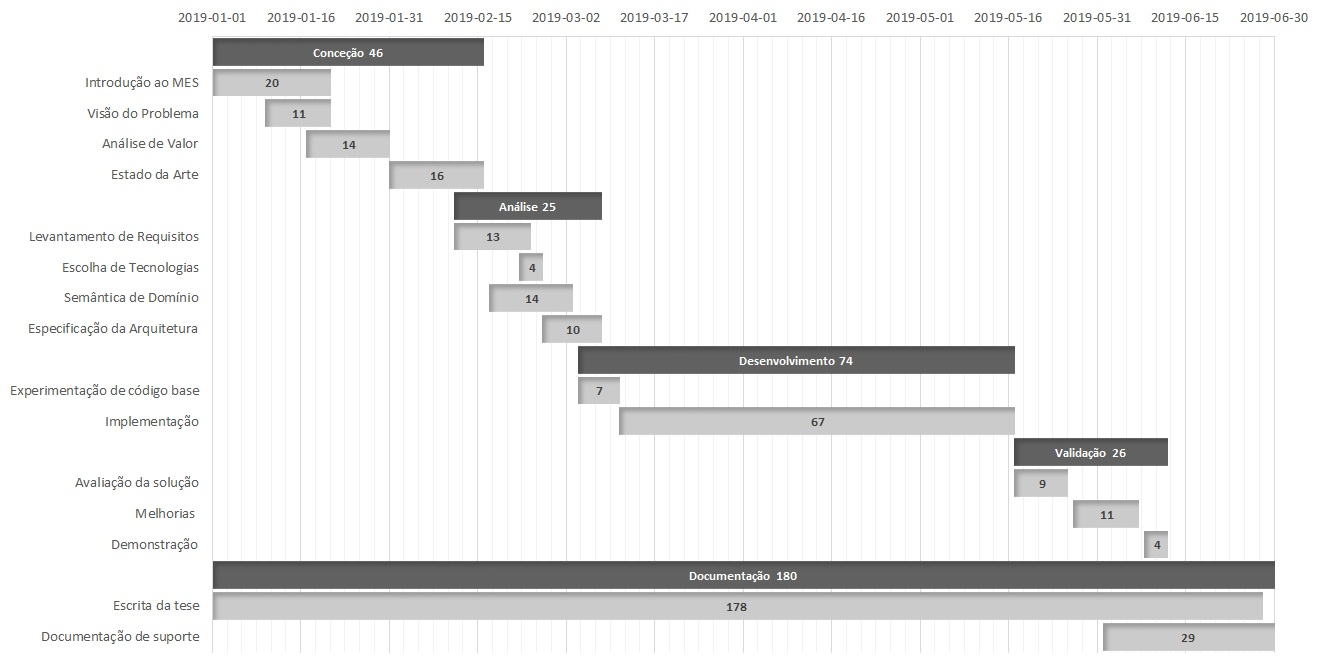
\includegraphics[width=1.0\textwidth]{pre-thesis/assets/gantt.jpg}
    \caption{Diagrama de \textit{Gantt} referente ao planeamento do projeto}
    \label{fig:planning-gantt_chart}
\end{sidewaysfigure}
\clearpage
